\section{Detector design}\label{sec:detector}


\subsection{Water Cherenkov Detector}

Thanks to its low cost, robustness, reliability and reasonable efficiency, on the of the most commonly used particle detectors in Astroparticle physics are the Water Cherenkov Detectors, with typical detection masses from one to thousands tons of water. The passage of ultra-relativistic charged particles through the water volume produce Cherenkov radiation mainly in 


that is collected by a central photomultiplier tube (PMT), typically an
8-inch Hamamatsu R5912 PMT. The sensitivity to secondary gammas in the cascade
is enabled by the production of Cherenkov capable electron/positron pairs




Based on the geographical distribution of the sites where LAGO operates, the basic design principles for LAGO detectors are simple: we focus on the utilization of low cost and low power consumption off the shelf components. The LAGO smart WCD are built starting from commercial polyethylene water tanks with $\sim 1$\,m$^3$ to $40$\,m$^3$ of purified water. 




The passage of
ultra-relativistic charged particles through the water volume produce Cherenkov
light that is collected by a central photomultiplier tube (PMT), typically an
8-inch Hamamatsu R5912 PMT. The sensitivity to secondary gammas in the cascade
is enabled by the production of Cherenkov capable electron/positron pairs
within the water volume. The detector has an internal coating made by a highly
diffusive and reflective fabric of commercial
Tyvek\textregistered
%\footnote{http://bit.ly/1whxoph}
. The diffusion of
Cherenkov photons in the fabric surface reduce the signal dependence with the
secondary particle trajectory within the detector. A FPGA based, own designed
fast analog-to-digital conversion electronics allows the operation of up to
four independent detectors in a same site. This electronics is controlled by a
Raspberry Pi or similar device. Additionally, the station has a temperature and
atmospheric pressure sensor and a GPS board for time synchronization between
different LAGO sites. The power consumption of the station is less than $11$\,W
and is powered by solar panels and batteries. The LAGO WCD are characterized by
its low cost and reliability, and a schema of this detectors can be seen in
figure \ref{lago_wcd}.





Estos dispositivos detectan la
radiación Cherenkov producida por el paso de una partícula cargada con
velocidad mayor a la velocidad de la luz en el agua. Otra de las ventajas de
los WCD es su capacidad para detectar los fotones presentes de las
cascadas\,\cite{Allard2007,AllardEtal2008, AllekotteEtal2008}, que constituyen
el $\sim 70\%$ del total de partículas de la EAS. Con un metro cúbico de agua
se alcanzan altas probabilidades de conversión de un fotón en un par
$e^\pm$\,\cite{Asorey2012b}. En la figura\,\ref{WCDEsquema} se muestra un
esquema del detector típico utilizado en el proyecto LAGO. Alrededor del mundo
existen varias instalaciones de WCD dedicadas a la detección de GRB: INCA en
Chacaltaya-Bolivia $5200$\,m s.n.m.\,\cite{Cabrera1999}; Milagro en Nuevo
México-EE.UU. a $2650$\,m s.n.m.\,\cite{Atkins2004}; el Observatorio Pierre
Auger en Malarg\"ue-Argentina a $1400$\,m s.n.m.\,\cite{Abraham2004a}, y HAWC
en Sierra Negra-México, a $4500$\,m s.n.m\,\cite{Abeysekara2012}.

Los WCD del proyecto LAGO pueden tener variadas geometrías, y un esquema típico
se muestra en la figura \ref{WCDEsquema}. En general están construidos a partir
de un tanque comercial para almacenamiento de agua, con una capacidad de entre
$1$\,m$^{3}$ y $10$\,m$^{3}$, llenos de agua purificada. Cada WCD de LAGO
replica la idea de los WCD del Observatorio Pierre Auger de manera simplificada
y económica. La independencia en la detección de señales respecto a la
dirección de movimiento de las partículas se logra al tapizar internamente el
detector con Tyvek, un material altamente reflexivo y difusivo, que logra la
uniformización de la radiación Cherenkov en tiempos del órden de $15$\,ns luego
del ingreso de la partículas al detector\,\cite{Asorey2012b}. Las señales
luminosas son convertidas en señales eléctricas mediante un PMT de alta
sensibilidad, alta ganancia y alta linealidad. Las señales provenientes del PMT
son digitalizadas mediante una electrónica de diseño propio de la colaboración
LAGO. Estas placas utilizan conversores analógico-digitales rápidos (FADC, por
sus siglas en inglés, \textit{Fast ``flash'' analog-to-digital converters}) con
una velocidad de muestreo de $40$\,MHz y con una resolución de $10$\,bits. Las
placas permiten además controlar las tensiones de polarización del PMT, y
disponen de tres canales independientes de digitalización y control. Se utiliza
una FPGA (\textit{Field Programmable Gate Array}) Digilent Nexys-II para el
control del GPS, del sensor de Presión y Temperatura y de la electrónica de
adquisición. Las señales digitales son procesadas por la FPGA y transferidas a
una computadora por el puerto USB. Esto dificulta la adquisición en sitios
remotos por el alto consumo de la PC de adquisición, y es por ello que en esta
propuesta se estudia la implementación de dispositivos de bajo consumo para el
control y almacenamiento de datos (Raspberry Pi y dispositivos de
almacenamiento de estado sólido). Una descripción completa del funcionamiento
de los WCD y de grandes arreglos de detectores puede consultarse
en\,\cite{Asorey2012b}.

La técnica utilizada por la colaboración LAGO para detectar GRB y fenómenos
solares es conocida como la técnica de partícula individual
(SPT)\,\cite{Vernetto2000}. Esta técnica se fundamenta en la detección de una
elevación en la tasa de conteo sobre un fondo base, en escalas de tiempo
relacionadas con los fenómenos a observar (desde algunos segundos para GRB
hasta semanas para la recuperación del flujo de secundarios luego de un FD).
Estas variaciones en el flujo de secundarios pueden ser correlacionados con
variaciones en el flujo de primarios en el límite superior de la atmósfera.
Esta técnica ha sido utilizada con éxito para la detección de fenómenos solares
en el observatorio Auger\,\cite{ThePierreAugerCollaboration2011,Asorey2011a}.
La SPT es, hasta ahora uno de los pocos métodos para detectar GRB en el rango
de los GeV, y puede verse una descripción completa aplicada a LAGO por
\cite{BertouAllard2005}. La elevación de un conteo de base en $5 \sigma$
durante un segundo representa un aumento de $\approx 270$ partículas\,m$^{-2}$
y a $5300$\,m s.n.m. un fotón de 100 GeV produce $\approx 290$
partículas\,m${-2}$, con lo cual un fotón de esa energía podría ser detectado
con un WCD de sólo $1$\,m$^2$ de superficie\cite{BertouAllard2005}. Por ello la
colaboración LAGO apunta a colocar detectores en elevaciones, por cuanto
$10$\,m$^{2}$ de WCD en $5300$\,m s.n.m. tienen la misma sensibilidad para
búsqueda de GRB que toda la instalación del Observatorio Pierre Auger con
$16000$\,m$^{2}$ de superficie de
detección\,\cite{AllardEtal2009A,AllardEtal2009B}.

A más altas energías, la dispersión lateral de las partículas en las EAS hace
que puedan encontrarse partículas provenientes de una misma cascada, y por lo
tanto correlacionadas, a cientos de metros y hasta algunos kilómetros de la
dirección de propagación de la partícula primaria. Por lo tanto, al disponer de
un arreglo de detectores espacialmente separados y temporalmente sincronizados
es posible muestrear la distribución lateral de las partículas en la lluvia.
Esto permite buscar correlaciones espacio-temporales entre las señales de los
distintos detectores, lo cual a su vez posibilita la triangulación de las
señales y sus intensidades, y de esta manera reconstruir la dirección de arribo
y la energía del rayo cósmico incidente\,\cite{Asorey2005}. La sincronización
temporal requerida es de algunos nanosegundos entre detectores separados a
algunos kilómetros, lo cual puede lograrse de manera simple, económica y
eficiente usando receptores GPS comerciales funcionando en el modo
{\textit{pulso por segundo}}\,\cite{Pryke1995}.

\begin{figure}
  \begin{center}
    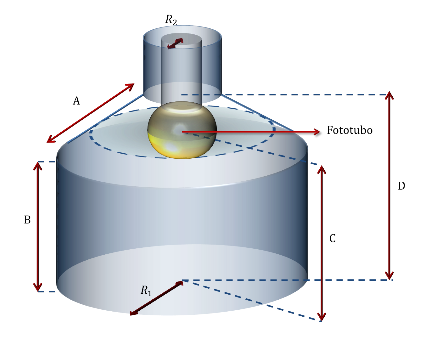
\includegraphics[width=0.4\textwidth]{images/detector.png}
    \caption{Esquema de un WCD típico de LAGO. El detector está formado por un
tanque plástico o metálico comercial de geometría cilíndrica o cilindro-cónica
y dimensiones variables, que contiene entre $1$\,m$^3$ y $10$\,m$^3$ de agua en
su interior. El pasaje de partículas cargadas ultra-relativistas por el agua
produce radiación Cherenkov en el interior del detector. Esta radiación es
reflejada y difundida gracias a un recubrimiento interno hecho de Tyvek. Luego,
un tubo fotomultiplicador de entre $6$\" y $9$\" capta la radiación Cherenkov y
la convierte en señales eléctricas, que luego son digitalizadas, procesadas y
almacenadas para su posterior análisis.} \label{WCDEsquema}
  \end{center}
\end{figure}

\subsection{Description of the data acquisition electronics}\label{sec:electronics}

A WCD is composed by a tank of water with a reflective material inside, and a
photomultiplier tube (PMT) to convert Cherenkov radiation produced by the
interaction of the high energy particles with water in an electric signal. The
response of each WCD, like other particle detectors, are short electric pulses
that are recorded by high speed data acquisition systems.

\subsubsection*{Bariloche design}

The PMT is connected to a electronic board, that have a voltage divider, a high
voltage supply, and an amplifier of the output pulse. The high voltage supply
can be controlled typically from 0\,V to 2000\,V with a signal from 0\,V to
5\,V. The output pulse shape of the PMT depends on the geometry of the tank,
for a tank of 1000\,l the FWMH (Full Width at Half Maximum) of the pulse is
around 150\,ns. At the same time, it is necessary to measure other information
relevant to the experiment, like pressure, temperature and PPS (Pulse Per
Second) from the GPS. The data acquisition and high voltage parameters of the
experiment can be settled by a PC program and the acquire pulses are transfered
in real time to the PC via a USB interface. This system has the capabality of
acquire three independent channels of pulses and provide the control signal for
the three HV supply.  Figure \ref{fig:electronic-b}, top, shows a block diagram
of the data acquisition system.

The data acquisition system includes a custom electronic board that integrate
the front-end electronics: three ADC, anti-aliasing filters, baseline control
control circuit, high voltage control signal, and the necessary service
circuits. This board is connected to a NEXYS-2 board \cite{nexys2} via a high
speed FX2-Hirose connector. The NEXYS2 have a FPGA Spartan3E that is connected
to the PC with a USB interface. The USB interface between the PC and the FPGA
is managed with a Cypress chip included in the board. In the FPGA there is an
implementation of a module of command, that provided connectivity with the
sensors the GPS and with a pre-processor that filter the input pulses. The
pulses that have an amplitude over a trigger level are transferred to the PC.
Every time that a PPS from the GPS occurs, the systems sends to the PC the
values of the preassure, temperature and the UTC time from the GPS. There is
also an implementation of a stabilizer circuit for the baseline.

A sub-trigger mode was specially developed for LAGO, it makes possible to
acquire only the amplitude and charge value of pulses that have amplitude above
a pre-seted value of ''sub-trigger''. With this feature is possible to  record
a high rate 100KHz of pulses without loss of data. This makes possible do a
classification in energy versus particle rate for the study of  solar physics
\cite{asorey:13}. For the proper operation of the sub-trigger mode, it is
necessary to get a stable baseline. A stabilizer circuit of the baseline is
implemented.

In figure \ref{fig:electronic-b}, bottom, a casing with the whole LAGO
electronic can be seen with the different components. The NEXYS-2 board with a
sensor for pression and temperature (HP03S), a switching power supply and a
digitalized board with three available channels.

\begin{figure}[htp!]
 \centering
 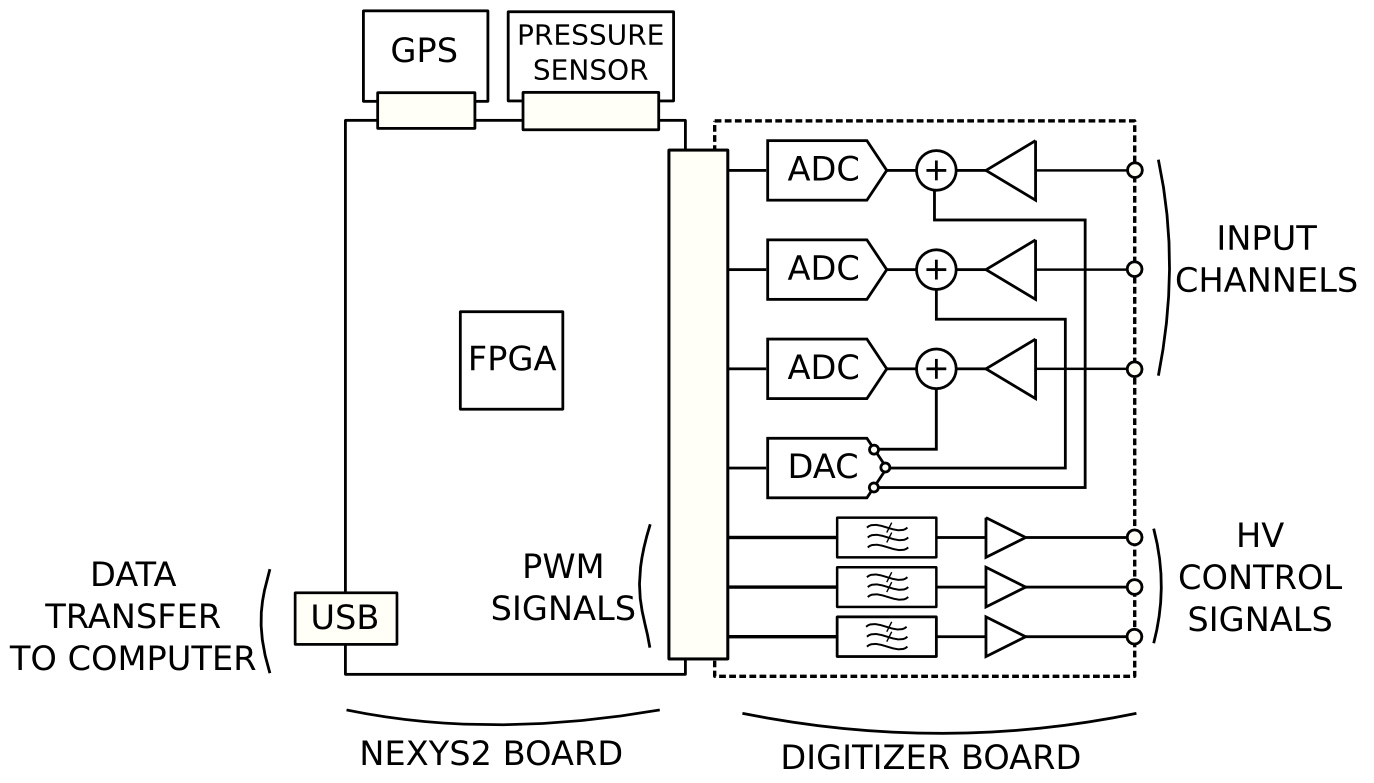
\includegraphics[width=0.65\textwidth,height=0.25\textheight]{images/bloques_electronica.png}
 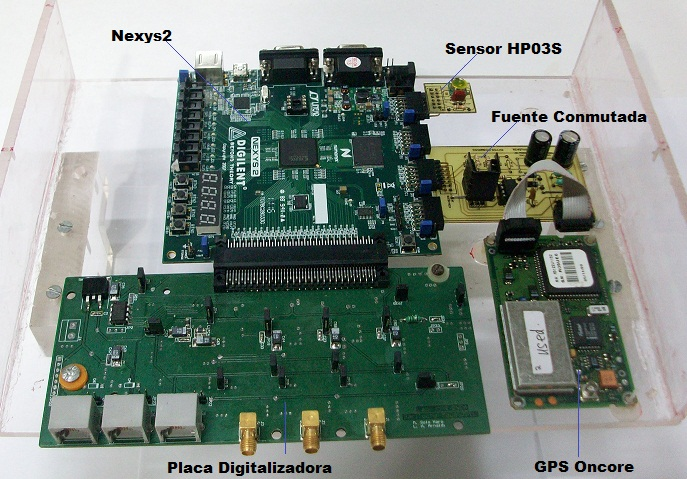
\includegraphics[width=0.70\textwidth,height=0.30\textheight]{images/venezuela/nuevaLS.jpg}
 \caption{Top: block diagram of the DAQ developed by LAGO Bariloche. Bottom:
Electronic kit designed for the LAGO collaboration, in the version assembled by
LAGO Venezuela} \label{fig:electronic-b}
\end{figure}  

\subsubsection*{Mexico design}

Field programmable gate arrays (FPGAs) was playing an increasing role in DAQ
systems in cosmic rays experiments due to their high speed and integration and
their low cost and low power consumption. Modern electronics based on on-chip
fast analog to digital converters (ADCs) and powerful digital signal processors
(DSPs) was being  ideal to be the basis of custom-made DAQ systems which are
more flexible, faster and cheaper than the traditional DAQ systems based on
modular electronics \cite{all:09}. We took advantage of these recent
developments, in particular in the area of very high integrated circuits in the
form of ADCs and FPGAs for the design of the new system which consisted of an
ADC daughter board running at 200 MSPS\footnote{Mega Samples Per Second}. Each
event was tagged with precise GPS time using a GPS embedded receiver with 1 PPS
(one pulse per second) synchronised with the atomic clock on the GPS satellites
within a corrected uncertainty of 50\,ns (Motorola Oncore UT+ module)\ref{ref}.
A pressure and Temperature sensor (HP03D) was adapted to the FPGA board (2FT
Xilinx).

% A picture of the final setup in its RF box is visible in figure
%\ref{fig:electronic-m}.

%\begin{figure}[t]
%\centering
%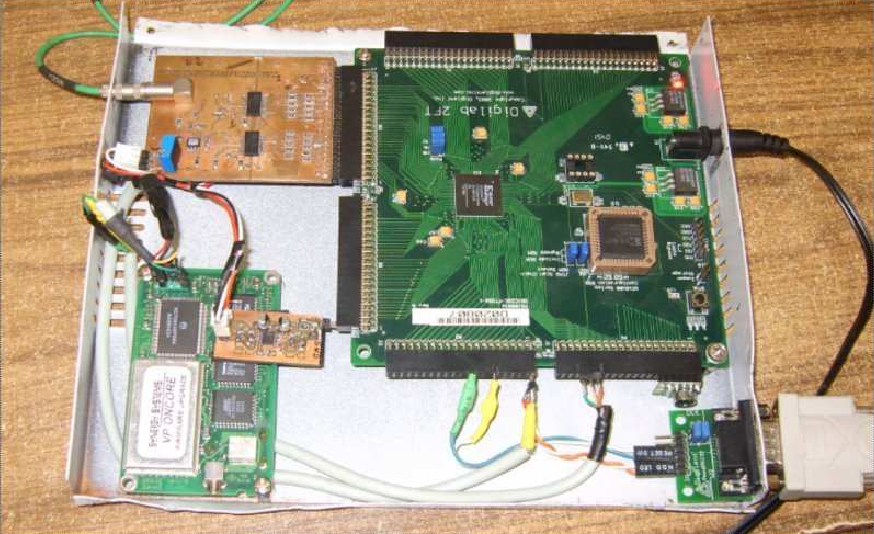
\includegraphics[scale=0.4]{images/mexico/sitelago-0A.png}
%\caption{New electronics for LAGO. The prototype can be operated at 100 or 200 MSPS.}
%\label{sitelago0A}
%\end{figure} 

The custom-made instrumentation for the DAQ system uses low power consumption,
it includes: A 4-channel ADC daughter-board with two dual 10-bit ADC chip
from Analog Devices, this chip was the AD9216 that is a dual, 3 V, 10-bit,
105 MSPS analog-to-digital converter. The daughter-board is connected to a
second board with an FPGA, for real-time data processing (Nexys2 from Digilent
Inc.); This board is a powerful digital system design platform built around a
Xilinx Spartan 3E FPGA, with 16 Mb of fast SDRAM and 16 Mb of Flash ROM. The
Nexys2 board is ideally suited to embedded processors like Xilinx's 32-bit
RISC Microblaze. Communication and control are based on a small minicomputer
Raspberry PI model B 512MB with an ARM1176JZF-S 700 MHz processor, this mini-
computer is the main control between the host y the DAQ, and it is used for
interconnection with the surface detector modules, the mother board has two
ways of communication with the host, the first one uses a serial port with a
typical communication rate around 115200 bits per second and the second one
uses a USB port with a higher communication speed.

A pressure and temperature sensor, (HP03D from Shenzhen Hope Microelectronics
Co. Ltd.) which includes a piezo-resistive pressure sensor and an ADC interface,
providing 16 bit word data for pressure and temperature related voltage, is
connected to the FPGA board. The algorithms developed use advanced digital
signal processing techniques and particularly digital pulse processing, where
the purpose of the pulse processing is to perform on-line signal processing
on the digitized signals directly to minimize the data transfer size, these
algorithms are implemented on the FPGA using Hardware Description Language
(VHDL) and C Language for the Microblaze processor, these algorithms can be
reprogrammed at any time. Each event is tagged with precise GPS time tags using
an embedded GPS receiver with 1 PPS (one pulse per second) synchronized with
UTC within an uncertainty of 50 ns (Motorola Oncore UT+ GPS receiver), see
figure \ref{fig:electronics-m}. The bitstream firmware of the DAQ system
resides permanently on the Flash ROM chip located on the mother board and it
gets downloaded into the FPGA upon power on.

%On the PC side we use Perl and Python under Linux to process,
%store and display the data acquired. Finally, we use ROOT programs to histogram
%and analyze the data.

\begin{figure}[t]
\centering
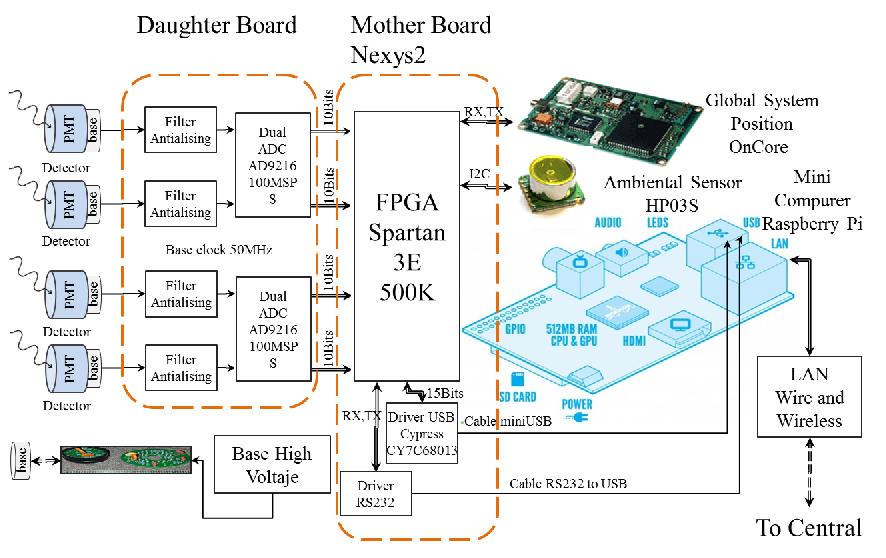
\includegraphics[scale=0.5]{images/mexico/sitelago-02.png}
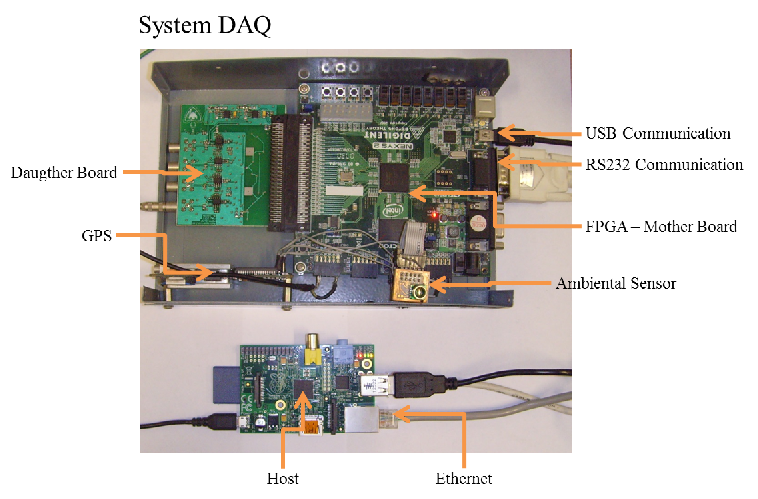
\includegraphics[scale=0.69]{images/mexico/sitelago-03.png}
\caption{Top: DAQ full blocks diagram, you can see the main parts of the DAQ.1.- Daughter Board 2.- Mother Board, and 3.- Host. Bottom: custom electronics designed for the LAGO mexican part of the collaboration, it can be operated at 100 or 200 MSPS}
\label{fig:electronics-m}
\end{figure} 

